\documentclass[a4paper,12pt]{article}

\usepackage{../usfdvl}


\title{Worksheet 4}
\SetDocumentFooter{}{}


\begin{document}

\maketitle

\worksheetGroundRules

\worksheetSubmission

\assignmentInstructions

\begin{enumerate}


\item For the following polygon draw all \textit{possible} diagonals from $A$ and $B$. For each possible diagonal, test if it is valid. if not, state the reason. 

\vspace{20pt}
\begin{center}
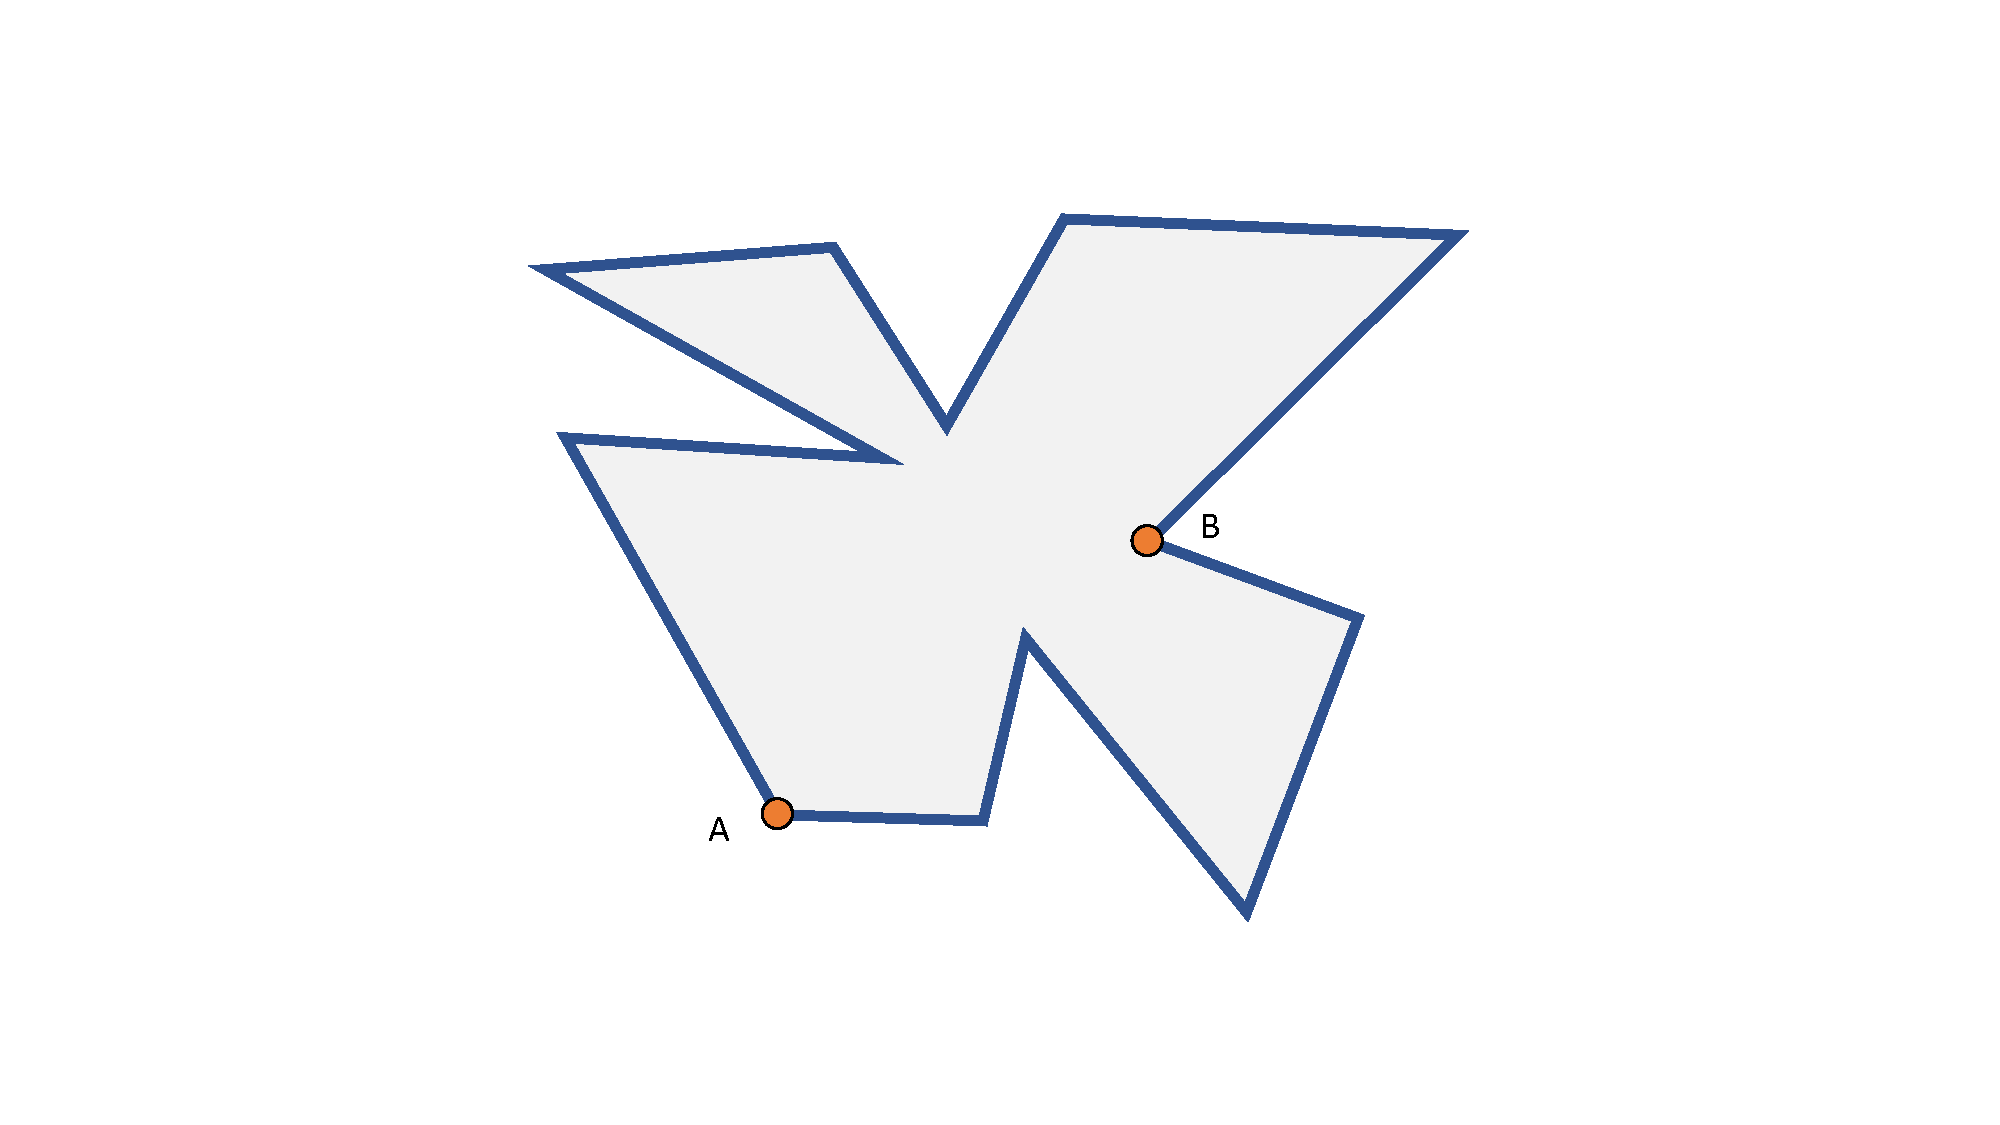
\includegraphics[width=0.8\linewidth]{../images/diagonals.pdf}
\end{center}


\newpage

\item For the following polygon show how you would determine if $C$ and $D$ are inside or outside of the polygon.

\vspace{20pt}
\begin{center}

\includegraphics[width=0.7\linewidth]{../images/point_in_poly.pdf}
\end{center}

\newpage

\item For the following polygon show how you would calculate the area of the polygon.

\vspace{20pt}
\begin{center}
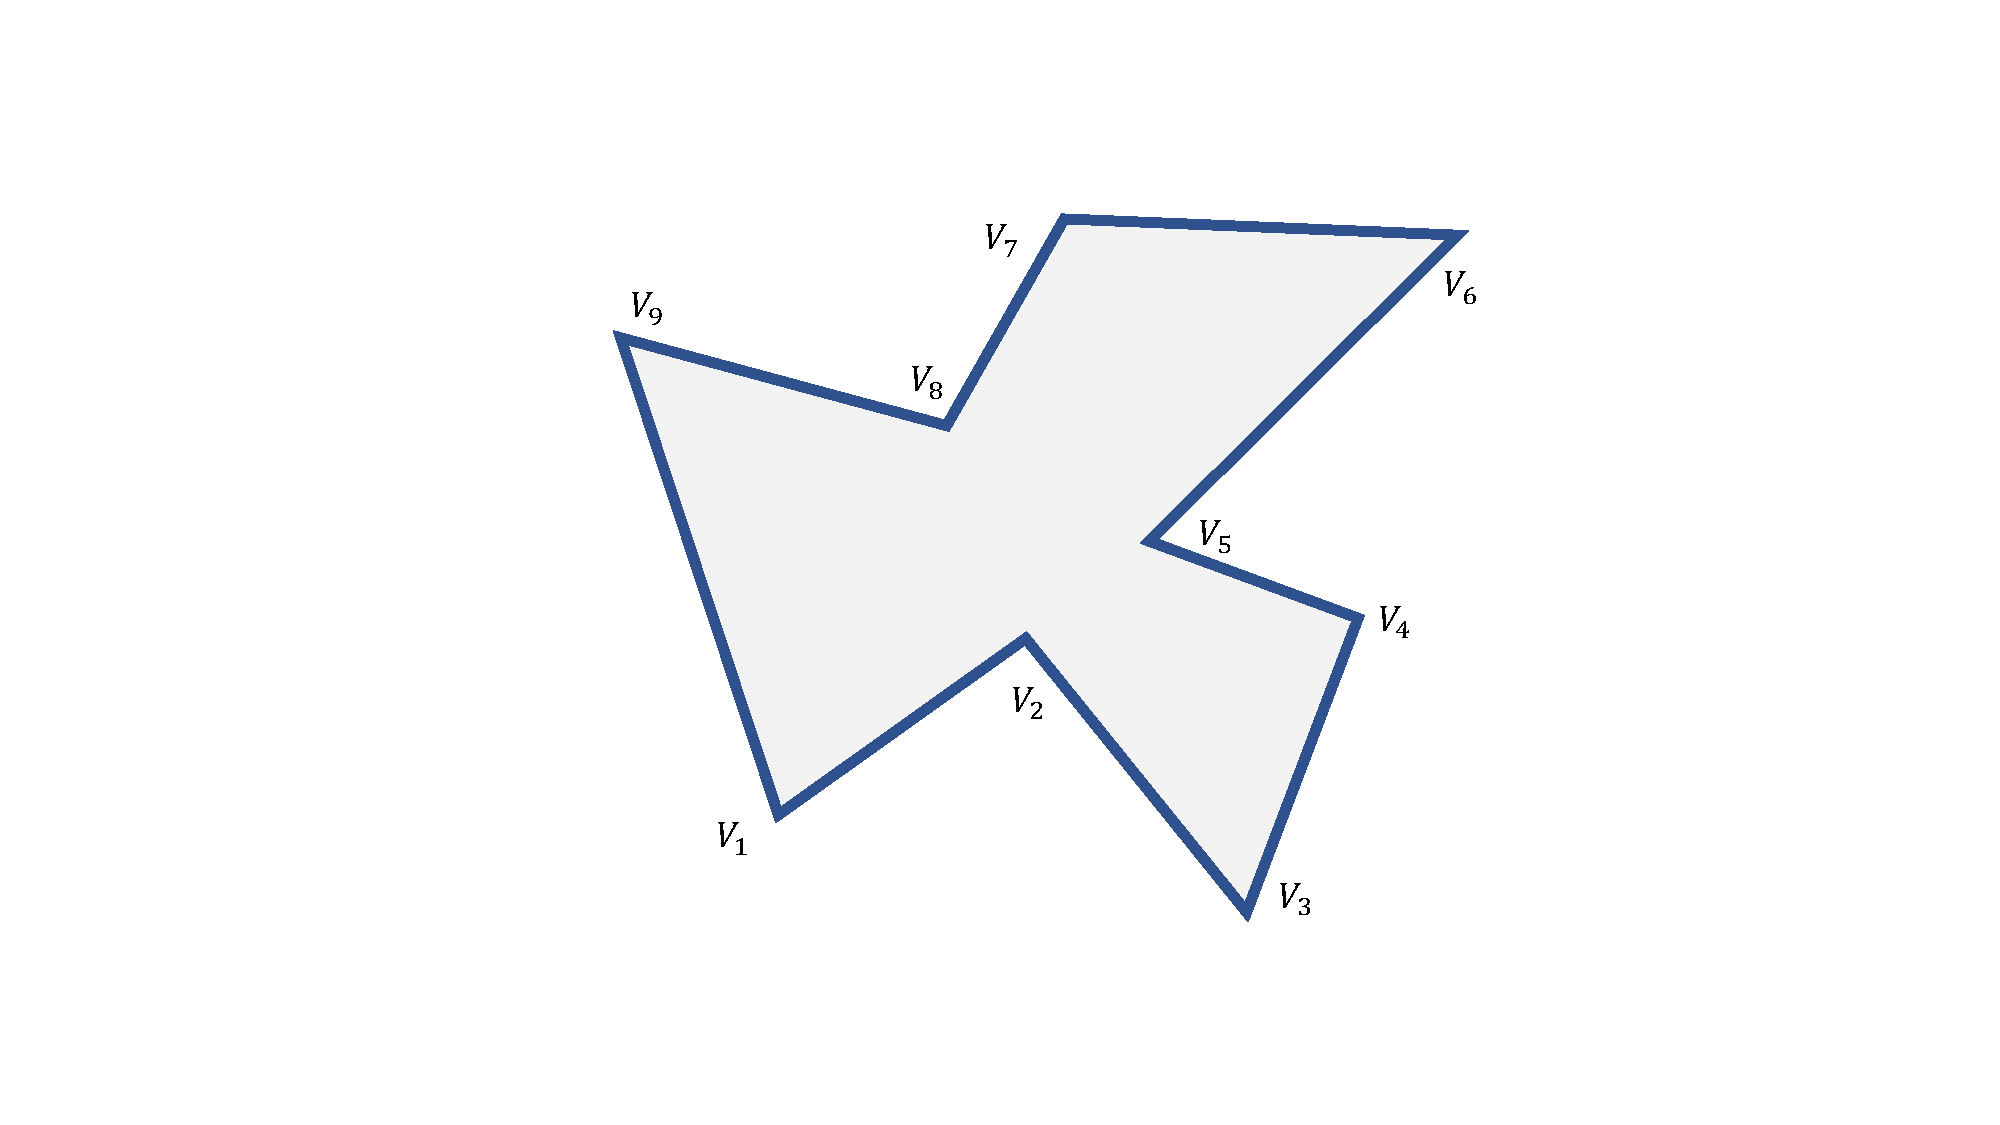
\includegraphics[width=0.7\linewidth]{../images/polygon_area.pdf}
\end{center}

\end{enumerate}


\end{document}

